
 \section{Modélisation 3D}
 %%%%%%%%%%%%%%%
 % Frame Section title
 \begin{frame}
 \title{Reconstruction 3D}
 \titlepage

    \begin{minipage}{0.3\textwidth}
    \begin{flushleft} \large
    \emph{Binôme :}\\
    B. Giraud\\
    M. Xu
    \end{flushleft}
    \end{minipage}
    \begin{minipage}{0.5\textwidth}
    \begin{flushright} \large
    \begin{figure}
    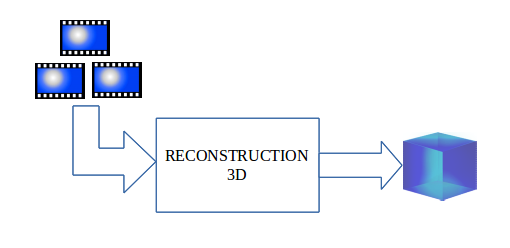
\includegraphics[width=1.4\textwidth]{Fig/architectureSectionReco3d.png}
    \end{figure}
    \end{flushright}
    \end{minipage}\\[3cm]
    
 \end{frame} 
 
\subsection{Architecture du programme}
 %%%%%%%%%%%%%%%
 % Frame Architecture inpainting
\begin{frame}
  \frametitle{Architecture du programme}
  \insertF{Fig/architectureReco3d.png}{Architecture de la partie Reconstruction 3D}{1}

\end{frame}	  
	  
	  
	  
	  
	  \subsection{Traitement}
	  %\subsection{Bundler}
	  
	  \begin{frame}
	  \frametitle{VisualSFM}
	   VisualSFM:
	  \begin{itemize}
	    \setbeamertemplate{itemize item}[triangle]
	    \item Calcule les SIFT pour trouver des correspondances
	    
	    \setbeamertemplate{itemize item}[triangle]
	    \item Estime la position des caméras
	    
	    \setbeamertemplate{itemize item}[triangle]
	    \item Calcule un nuage de points 3D dense
	    \end{itemize}
	    
	   \insertF{Fig/nuagePtsTemple4coup.png}{Nuage de points}{0.4}

	  \end{frame}
	  	  
	  %\subsection{MeshLab}
	  
	  \begin{frame}
	  \frametitle{MeshLab}
	    MeshLab:
	  \begin{itemize}
	    \setbeamertemplate{itemize item}[triangle]
	    \item Récupère le nuage de points calculé
	    
	    \setbeamertemplate{itemize item}[triangle]
	    \item Construit un maillage
	    
	    \setbeamertemplate{itemize item}[triangle]
	    \item Calcule une couleur par sommet du maillage
	    \end{itemize}
	    
  \begin{figure}
  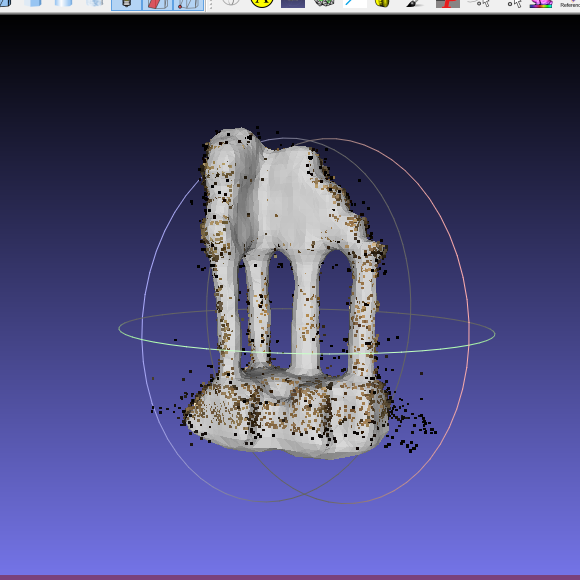
\includegraphics[width=0.45\textwidth]{Fig/nuagePtsTemple6coup.png}
  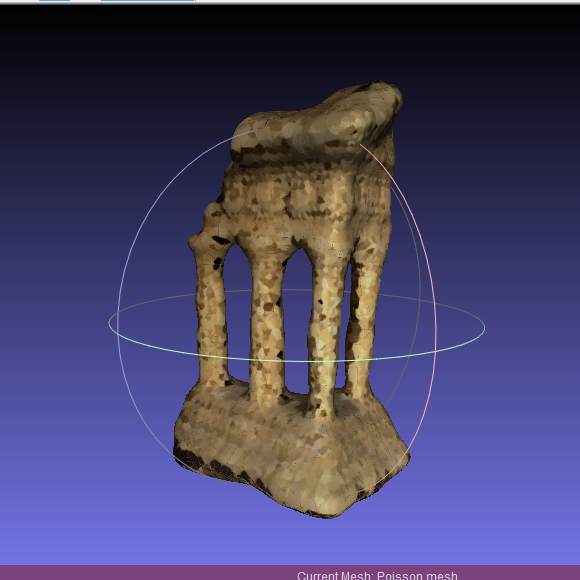
\includegraphics[width=0.45\textwidth]{Fig/nuagePtsTemple8coup.png}
  \caption{Reconstruction du maillage}
  \end{figure}
  
	 \end{frame}

	 \subsection{Sortie}
	 \begin{frame}
	  \frametitle{Sortie du programme}
	   Nous avons donc en sortie:
	  \begin{itemize}
	    \setbeamertemplate{itemize item}[triangle]
	    \item Un maillage avec les couleurs par scène données en entrée.
	    
	    
	    \end{itemize}
	 \end{frame}

 %%%%%%%%%%%%%%%
  % Frame demonstration
 \begin{frame}
   \frametitle{Démonstration}
   \begin{figure}
   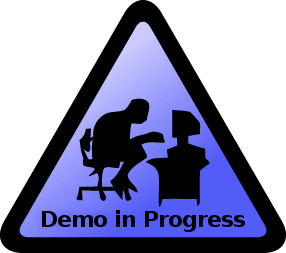
\includegraphics[width=0.5\textwidth]{Fig/demoInProgress.png}
   \end{figure}

 \end{frame}